\subsection{Communication between PL and PS}
Sending thresholds from the processing system to the PWM low-level modules are done through a piece of block RAM.
The build-in block RAM of the Zybo consist of a 36kbit storage area with two independent access ports. 

The PWM modules expect 8 bit thresholds which results in 24 bits or 3 bytes being used of the block RAM. 

A mere 3 bytes account for around $0.08\%$ of the total block RAM. While this is a waste of the block RAM, it was chosen because of it being easily accessible from both the PS and PL and easy to set up. 

When the control task on the processing system has run and produced the thresholds for each phase they are written into the first 3 bytes of the block RAM as can be seen on figure \ref{fig:com_pl_to_ps}.

\begin{figure}[H]
	\centering
	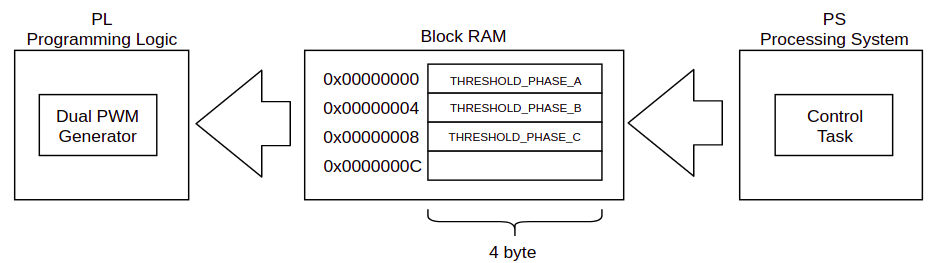
\includegraphics[width=1\linewidth]{pictures/software/com_pl_to_ps.png}
	\caption{Communication from PS to PL through block RAM.}
	\label{fig:com_pl_to_ps}
\end{figure}

From here the memory interface module in the logic can collect the thresholds and parse them unto the three PWM modules as can be seen on figure \ref{fig:com_pl}. The PWM modules then use the thresholds to produce the PWM signals as discussed in section \ref{sec:pwm}.


\begin{figure}[H]
	\centering
	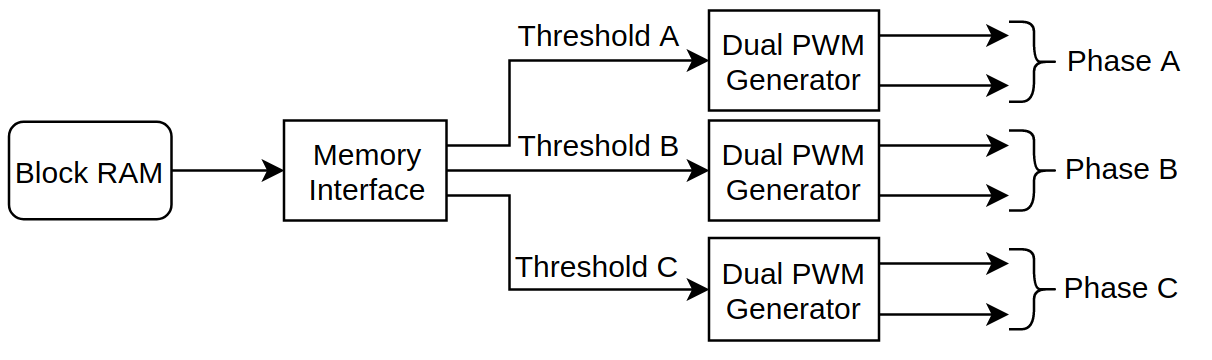
\includegraphics[width=0.8\linewidth]{pictures/software/com_pl.png}
	\caption{The data flow in the PL from the block RAM to the PWM generators.}
	\label{fig:com_pl}
\end{figure}


